

\tikzset{every picture/.style={line width=0.75pt}} %set default line width to 0.75pt        

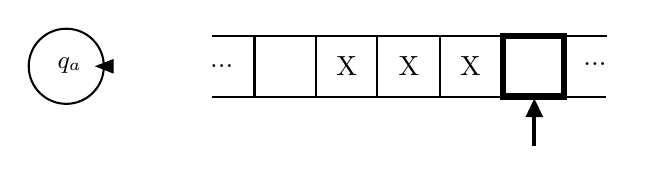
\begin{tikzpicture}[x=0.75pt,y=0.75pt,yscale=-1,xscale=1]
%uncomment if require: \path (0,446); %set diagram left start at 0, and has height of 446

%Shape: Triangle [id:dp9549836358247636] 
\draw  [fill={rgb, 255:red, 0; green, 0; blue, 0 }  ,fill opacity=1 ] (134.4,85) -- (141.6,82.2) -- (141.6,87.8) -- cycle ;
%Shape: Circle [id:dp39324764126664746] 
\draw   (101.2,85) .. controls (101.2,75) and (109.31,66.9) .. (119.3,66.9) .. controls (129.3,66.9) and (137.4,75) .. (137.4,85) .. controls (137.4,95) and (129.3,103.1) .. (119.3,103.1) .. controls (109.31,103.1) and (101.2,95) .. (101.2,85) -- cycle ;
%Straight Lines [id:da279972863636345] 
\draw    (379.6,70.2) -- (248.8,70.2) -- (189.6,70.2) ;
%Straight Lines [id:da8063028764122899] 
\draw    (379.2,99.6) -- (189.4,99.6) ;
%Straight Lines [id:da6194955219154272] 
\draw    (210,70.4) -- (210,99.6) ;
%Straight Lines [id:da9291793988668682] 
\draw    (239.6,70.8) -- (239.6,100) ;
%Straight Lines [id:da1753997056206802] 
\draw    (269.2,70.4) -- (269.2,99.6) ;
%Straight Lines [id:da7326138590955908] 
\draw    (299.2,70.4) -- (299.2,99.6) ;
%Straight Lines [id:da8827634409952425] 
\draw    (329.2,70.4) -- (329.2,99.6) ;
%Straight Lines [id:da08240500809926843] 
\draw    (359.2,70.8) -- (359.2,100) ;
%Shape: Rectangle [id:dp8505881042891044] 
\draw  [line width=2.25]  (359.2,99.6) -- (329.6,99.6) -- (329.6,70.4) -- (359.2,70.4) -- cycle ;
%Straight Lines [id:da2295782410185434] 
\draw    (344.8,117.75) -- (344.8,103.55) ;
\draw [shift={(344.8,100.55)}, rotate = 90] [fill={rgb, 255:red, 0; green, 0; blue, 0 }  ][line width=0.08]  [draw opacity=0] (8.93,-4.29) -- (0,0) -- (8.93,4.29) -- cycle    ;
%Straight Lines [id:da2131860495885145] 
\draw [line width=1.5]    (344.8,123.4) -- (344.8,106.15) ;


% Text Node
\draw (107.4,79.2) node [anchor=north west][inner sep=0.75pt]  [font=\small] [align=left] {\begin{minipage}[lt]{18.04pt}\setlength\topsep{0pt}
\begin{center}
$q_\text{a}$
\end{center}

\end{minipage}};
% Text Node
\draw (224.8,85.4) node   [align=left] {\begin{minipage}[lt]{20.13pt}\setlength\topsep{0pt}
\begin{center}
\Vtextvisiblespace
\end{center}

\end{minipage}};
% Text Node
\draw (254.4,85) node   [align=left] {\begin{minipage}[lt]{20.13pt}\setlength\topsep{0pt}
\begin{center}
X
\end{center}

\end{minipage}};
% Text Node
\draw (284.4,85) node   [align=left] {\begin{minipage}[lt]{20.13pt}\setlength\topsep{0pt}
\begin{center}
X
\end{center}

\end{minipage}};
% Text Node
\draw (314,85) node   [align=left] {\begin{minipage}[lt]{20.13pt}\setlength\topsep{0pt}
\begin{center}
X
\end{center}

\end{minipage}};
% Text Node
\draw (344.4,85.4) node   [align=left] {\begin{minipage}[lt]{20.13pt}\setlength\topsep{0pt}
\begin{center}
\Vtextvisiblespace
\end{center}

\end{minipage}};
% Text Node
\draw (374,85.4) node   [align=left] {\begin{minipage}[lt]{20.13pt}\setlength\topsep{0pt}
\begin{center}
...
\end{center}

\end{minipage}};
% Text Node
\draw (194.2,86) node   [align=left] {\begin{minipage}[lt]{20.13pt}\setlength\topsep{0pt}
\begin{center}
...
\end{center}

\end{minipage}};


\end{tikzpicture}
